\chapter{\IfLanguageName{dutch}{Stand van zaken}{State of the art}}
\label{ch:stand-van-zaken}

% Tip: Begin elk hoofdstuk met een paragraaf inleiding die beschrijft hoe
% dit hoofdstuk past binnen het geheel van de bachelorproef. Geef in het
% bijzonder aan wat de link is met het vorige en volgende hoofdstuk.

% Pas na deze inleidende paragraaf komt de eerste sectiehoofding.

%Dit hoofdstuk bevat je literatuurstudie. De inhoud gaat verder op de inleiding, maar zal het onderwerp van de bachelorproef *diepgaand* uitspitten. De bedoeling is dat de lezer na lezing van dit hoofdstuk helemaal op de hoogte is van de huidige stand van zaken (state-of-the-art) in het onderzoeksdomein. Iemand die niet vertrouwd is met het onderwerp, weet nu voldoende om de rest van het verhaal te kunnen volgen, zonder dat die er nog andere informatie moet over opzoeken \autocite{Pollefliet2011}.

%Je verwijst bij elke bewering die je doet, vakterm die je introduceert, enz. naar je bronnen. In \LaTeX{} kan dat met het commando \texttt{$\backslash${textcite\{\}}} of \texttt{$\backslash${autocite\{\}}}. Als argument van het commando geef je de ``sleutel'' van een ``record'' in een bibliografische databank in het Bib\LaTeX{}-formaat (een tekstbestand). Als je expliciet naar de auteur verwijst in de zin, gebruik je \texttt{$\backslash${}textcite\{\}}.
%Soms wil je de auteur niet expliciet vernoemen, dan gebruik je \texttt{$\backslash${}autocite\{\}}. In de volgende paragraaf een voorbeeld van elk.

%\textcite{Knuth1998} schreef een van de standaardwerken over sorteer- en zoekalgoritmen. Experten zijn het erover eens dat cloud computing een interessante opportuniteit vormen, zowel voor gebruikers als voor dienstverleners op vlak van informatietechnologie~\autocite{Creeger2009}.

In dit hoofdstuk zal uitgelegd worden wat de huidige stand van zaken is van toegangssystemen bij de parking van UGent en welke andere technologieën hiervoor hedendaags gebruikt worden.
Verder wordt er besproken wat de GDPR inhoudt en waar deze op slaat. Ten laatste wordt er bekeken wat de voorgestelde hardware betreft voor dit onderzoek.

\section{Huidige situatie UGent}
% Huidige situatie UGent

Het huidige toegangssysteem aan UGent op de beschreven locaties is een systeem op basis van tokens. Een bezoeker rijdt de parking op zonder enige checks. Vervolgens bezoekt hij de campus en vraagt een token om de campus te verlaten. Ten laatste rijdt hij zijn wagen naar de slagboom en geeft zijn token in de gepaste tokenslikker.
Op de campus Sterre zijn er 3 ingangen en 2 uitgangen, op de campus Landbouw is dit gelijkaardig met 3 ingangen en 2 uitgangen.

\subsection{Technologieën in gebruik}
Meerdere toegangssystemen zijn vandaag de dag al in gebruik aan de campussen Landbouw en Sterre. Voor de toegang van personeel, studenten en bezoekers.

\subsubsection{Tokens}

%Hoe werken de tokens
Tokens worden aan alle uitgangen van de campussen gebruikt om de parking te verlaten.
Tokens worden hoofdzakelijk gebruikt om de parking te verlaten, alle uitgangen beschikken over een tokenslikker. Op deze manier kunnen studenten of bezoekers de campus verlaten nadat zij een token gaan afhalen op het onthaal.

%Nadelen van tokens
De tokens zelf vallen momenteel niet in goede aard omdat deze enkele nadelen met zich meebrengen:
\begin{itemize}
	\item De tokens worden veel misbruikt op faciliteiten buiten UGent zoals automaten, carwashes en meer.
	\item De tokens zelf kunnen makkelijk verloren geraken, wat niet milieubewust is.
	\item De tokens zelf redelijk duur aan een kost van 1,5 euro per stuk.
\end{itemize}

Deze punten geven aan dat tokens niet de gewenste oplossing zijn voor de campussen van UGent. Dit is te merken aan de hoofduitgang van de Campus Landbouw waar de uitgang vrij is om door te laten omdat de slikkers te veel werk met zich meebrengen.

\begin{figure}[h!]
	\centering
	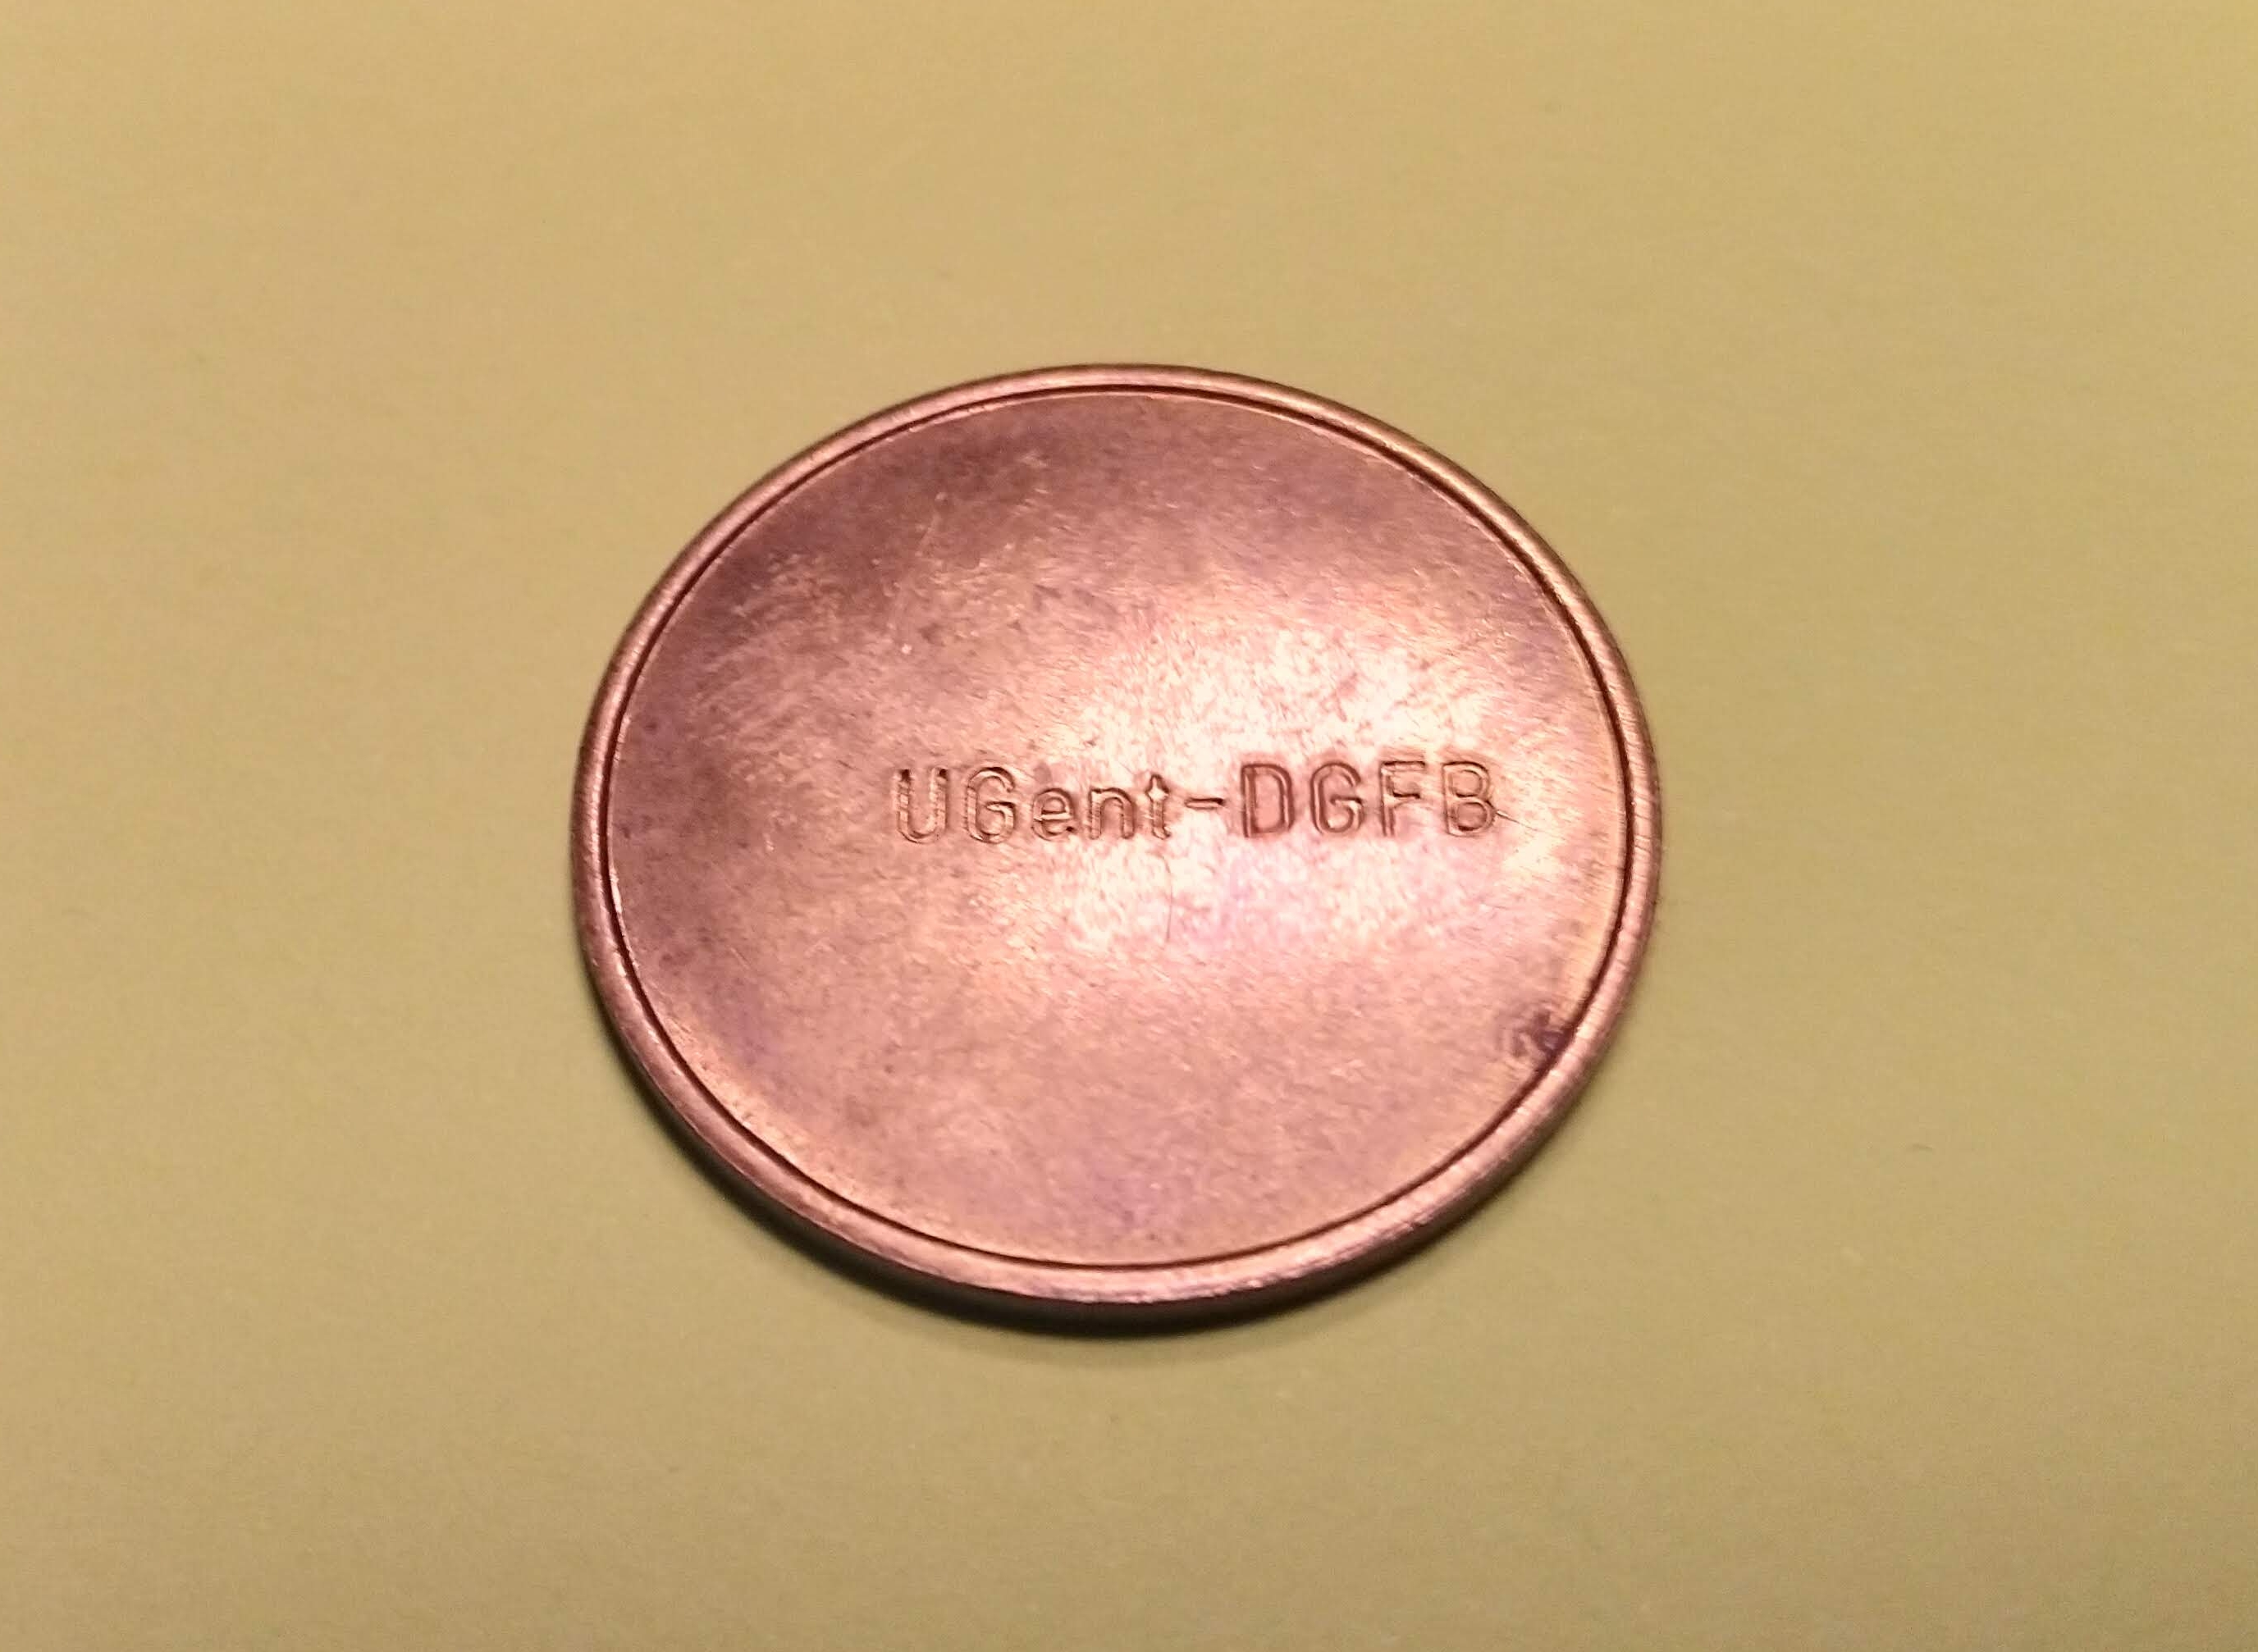
\includegraphics[width=0.5\linewidth]{img/token.jpg}
	\caption{Een huidige toegangstoken voor de parking van UGent te kunnen verlaten.}
\end{figure}

\subsubsection{Radio frequency Identification}

%Wat is RFID
Radio frequency Identication (RFID) is een technologie die aan de hand van elektromagnetische golven objecten kan identificeren. Dit met het voordeel dat er geen direct contact of zicht moet zijn tussen de scanner en het object. RFID gebeurt a.d.h.v een RFID reader en een RFID tag. De reader zendt een elektromagnetisch signaal uit. De tag ontvangt deze golven en kan op zijn beurt de opgevraagde informatie verzenden. \autocite{li2009design}

%RFID op UGent
Aan iedere uitgang op UGent zijn RFID-kaartlezers te vinden. Deze zijn voorzien om een vlotte toegang te verlenen aan werknemers en worden via een centraal systeem beheerd. Studenten en bezoekers hebben geen toegang tot dit systeem.
%TODO Gino vragen over exacte werking van de RFID op ugent

%TODO voordelen
Heel draagbaar, geen slikkers nodig.
%TODO nadelen
% \textcite{aalsalem2015automated} beschrijft wat onveilig is aan rfid. (kopieren van kaarten)
Het is geen optie om rfid voor alle bezoekers te gebruiken aangezien er vaak bezoekers binnentreden die maar 1 dag op de campus zijn. Aangezien er anders voor iedere dagbezoeker een RFID-kaart moet gemaakt worden is dit geen gewenste oplossing. Verder is de prijs van een RFID-kaart over de 10 euro, wat een te dure oplossing is.

\subsubsection{Barcodes}
In een poging tot de tokens te vervangen heeft UGent één uitgang op de parking UFO en het rectoraat waar barcodes worden gebruikt. Deze worden eerst geprint op de campus zelf, waarna de gebruiker de barcode in een slikker kan invoeren en toegang krijgen om de parking te verlaten.
%TODO gino vragen daar exacte werking barcode.

Deze barcodes hebben het voordeel dat ze goedkoper zijn om te maken per persoon. Voor de rest hebben ze nog steeds het probleem dat iedere gebruiker telkens aan het onthaal een nieuw ticket moeten opvragen en dat de slikkers geleegd moeten worden.

Nadelen:
\begin{itemize}
	\item Milieubelasting, verspilling van papier
	\item ofwel moet een papierslikker geledigd worden ofwel zal er vervuiling zijn van achtergelaten papier aan de uitgang.
	\item Op diverse plaatsen moeten er drukkers aanwezig zijn.
\end{itemize}


\subsection{Andere potentiele toegangstechnologieen}
De technologieen in gebruik op UGent zijn weliswaar niet de enigste toegangsstechnieken die bestaan.
%TODO bron andere toegangstechnieken

\subsubsection{ANPR}
Automatic Number Plate Recognition (ANPR) is de techniek om automatisch nummerplaten te herkennen. Deze techniek wordt al sinds 1976 gebruikt voor voor de detectie van gestolen wagens \autocite{uk2011anpr}. Hedendaags is ANPR al veel toegankelijker en kan het op vele plaatsen teruggevonden worden zoals bij bv. trajectcontrole \autocite{de2014snelheidscamera}, parkeersystemen, etc.
\par
ANPR heeft nog vele andere acroniemen zoals Automatic License Plate Recognition (ALPR), Automatic Vehicle Identification (AVI), Vehicle Plate recognition (VLPR), Vehicle Recognition Identifier (VRI), Car plate Recognition (CPR) en Car Plate Reader (CPR) \autocite{axis2019license}. In dit onderzoek zal voor nummerplaatdetectie het acroniem ANPR gebruikt worden.
\par
%Voordelen
Het gebruik van ANPR brengt enkele voordelen met zich mee:
\begin{itemize}
	\item Het is heel modulair; mensen kunnen een dagpas of toegang voor een volledig schooljaar krijgen.
	\item Er moet slechts éénmalig aangemeld worden om toegang voor een langere periode te krijgen. Dit zou helemaal digitaal gedaan kunnen worden, wat personeelskosten bespaart.
	\item Indien succesvol geïmplementeerd kan ANPR opstoppingen aan toegangspunten verminderen omdat er geen menselijke interactie met het systeem meer nodig is.
\end{itemize}
\par
%Nadelen
ANPR zelf komt ook met enkele nadelen.
\begin{itemize}
	\item Er is een centraal systeem nodig om de toegang van de nummerplaten te beheren.
	\item Ieder toegangspunt moet een internetvoorziening hebben om met het centrale systeem te communiceren.
	\item Iedere ANPR-camera moet correct ingesteld zijn om haalbare resultaten te behalen.
	\item Weersomstandigheden bieden extra moeilijkheid voor de detectie van nummerplaten (dag, nacht)
	\item Hedendaagse ANPR-camera's zijn een redelijke investering.
\end{itemize}
\par
Voor de herkenning van nummerplaten zijn een aantal technologien beschikbaar. Deze werken adhv. Artificial Intelligence (AI) en zijn specifiek getraint op het detecteren en uitlezen van nummerplaten.
De technologie die in dit onderwerp gebruikt zal worden is OpenALPR, een Open-Source library gemaakt voor nummerplaatdetectie. Hiervoor is gekozen omdat OpenALPR een gratis Open-Source product is \autocite{openalprgithub}.
%Nadelen


\section{Privacy en GDPR}
\label{sec:privacy-en-gdpr}
%TODO Privacy en gdpr onderdeel uitbreiden

Sinds 25 Mei 2018 is de General Data Protection Regulation (GDPR) in gang gezet, een regulatie die ingevoerd is om het huidige  en toekomstige digitale tijdperk veiliger te maken voor alle EU inwoners.
Deze wetgeving is gedreven op het concept dat privacy een mensenrecht is, en dat online-data ook zo behandeld moet worden. Dit is data die direct of indirect gelinkt kan worden aan een individu zoals locatie-data, cookies en ip-adressen \autocite{goddard2017eu}.

Hierdoor komen er een groot aantal extra regels op bedrijven te liggen, zo zijn ze bvb. verplicht om te toestemming vragen om persoonsgegevens te mogen verwerken. Dit is merkbaar online, waar vele sites toestemming vragen om advertentie-cookies te mogen opslaan. Een heleboel andere regels zijn er ook bijgekomen, wat het moeilijk kan maken om een nieuw systeem te maken die aan al deze voldoet.

\section{Hardware}
Om deze nummerplaatdetectie uit te voeren is gekozen voor een Raspberry PI Model B+. Deze hardware wordt vandaag de dag veel gebruikt bij IOT-applicaties door zijn lage kost en gemakkelijke bruikbaarheid.  

De Raspberry PI Model B+ beschikt over een 1.4GHz quad-core processor, 1GB LPDDR2 RAM, een on-board WiFi-kaart en de mogelijkheid om een Raspberry Pi Camera te verbinden \autocite{raspberrypisitemodelbplus} .

\subsection{Camera}
De camera die gebruikt wordt is een Pi-NoIr camera. Deze camera is ook geproduceerd door de Raspberry Pi Foundation en biedt afbeeldingen en video in een 8-MegaPixel formaat. In dit onderzoek is voor deze camera gekozen omdat deze makkelijk te verbinden is met de Raspberry Pi, relatief goedkoop is en geen IR-filter heeft. Dit maakt de camera direct ook interessant voor foto's te nemen in donkere omgevingen. \autocite{raspberrypisitemodelpinoir}